\documentclass[12pt]{article}

% Essential Packages
\usepackage{setspace}
\usepackage{pdfpages}
\usepackage{newtxtext} % Times New Roman
\usepackage[a4paper, left=3.5cm, top=2.5cm, right=1.5cm, bottom=2.85cm, includefoot]{geometry} % Margins
\usepackage{graphicx}
\usepackage[table]{xcolor}
\usepackage{tocbibind}
\usepackage{fancyhdr}
\usepackage[acronym]{glossaries}
\usepackage{url}
\usepackage{caption}
\usepackage{longtable}

\usepackage[T1]{fontenc} % Formatting
\usepackage[utf8]{inputenc}
\usepackage{csquotes}

% Optional packages
\usepackage{listings}% Code blocks with syntax highlighting:
\usepackage{hyperref} % PDF hyperlinks
\hypersetup{ % Set all link colours to black - clickable but inconspicuous
    colorlinks = true,
    citecolor = black,
    linkcolor = black,
    filecolor = black,
    urlcolor = black
}


% Thesis metadata
% ‼️‼️‼️‼️ Choose thesis type ‼️‼️‼️‼️
% Uncomment only one of the following lines:
%\def\isBachelorThesis{1} % Bachelor thesis
\def\isMasterThesis{1} % Master thesis

% If the thesis is in Slovak
\usepackage[english,main=slovak]{babel}
\def\secondlang{english}

% If the thesis is in English
%\usepackage[main=english,slovak]{babel}
%\def\secondlang{slovak}

\def\thesistitle{Názov práce}
\def\thesisauthor{Bc. Janko Mrkvička}

\def\uid{FI-123456-12345} % Replace with your own student ID
\def\supervisor{doc. RNDr. Severín Hrot, PhD.}
%\def\consultant{Mgr. Ignác Novák} % Optional, comment if not used
\def\thesisyear{2026}


% Load lang mutations
\addto\captionsenglish{
	\def\lndiplomathesis{Master's thesis}
	\def\lnbachelorthesis{Bachelor's thesis}
	\def\lnlistingname{Listing}
	\def\lnlistlistingname{List of Listings}
	\def\lnlistabbr{List of Abbreviations}
	\def\lnintro{Introduction}
	\def\lnconclusion{Conclusion}
	\def\lnbibliography{References}
	\def\lnkeywords{Keywords}
	\def\lnacknowledgement{Acknowledgement}
	\def\lnappendices{Appendices}
	\def\lndeclaration{Affidavit}
	\def\lndeclarationtext{I hereby declare that I have prepared this thesis independently and I have provided all the used literature.}
	\def\lnprogram{Program}
	\def\lnfieldofstudy{Field of study}
	\def\lndepartment{Department}
	\def\lnsupervisor{Supervisor}
	\def\lnconsultant{Consultant}
	\renewcommand{\contentsname}{Table of Contents}
	% University metadata
	\def\university{Pan-European University}
	\def\faculty{Faculty of Informatics}
	\def\program{Applied Informatics}
	\def\fieldofstudy{Informatics}
	\def\department{Institute of Applied Informatics}
}


\addto\captionsslovak{
	\def\lndiplomathesis{Diplomová práca}
	\def\lnbachelorthesis{Bakalárska práca}
	\def\lnlistingname{Výpis}
	\def\lnlistlistingname{Zoznam výpisov}
	\def\lnlistabbr{Zoznam skratiek a značiek}
	\def\lnintro{Úvod}
	\def\lnconclusion{Záver}
	\def\lnbibliography{Použitá literatúra}
	\def\lnkeywords{Kľúčové slová}
	\def\lnacknowledgement{Poďakovanie}
	\def\lnappendices{Prílohy}
	\def\lndeclaration{Čestné prehlásenie}
	\def\lndeclarationtext{Čestne vyhlasujem, že záverečnú prácu som vypracoval samostatne a že som uviedol všetku použitú literatúru.}
	\def\lnprogram{Študijný program}
	\def\lnfieldofstudy{Študijný odbor}
	\def\lndepartment{Školiace pracovisko}
	\def\lnsupervisor{Školiteľ}
	\def\lnconsultant{Konzultant}
	% University metadata
	\def\university{Paneurópska vysoká škola}
	\def\faculty{Fakulta Informatiky}
	\def\program{Aplikovaná informatika}
	\def\fieldofstudy{Informatika}
	\def\department{Ústav aplikovanej informatiky}
}


\title{\thesistitle}
\author{\thesisauthor}

% Bachelor thesis info
\ifdefined\isBachelorThesis
\def\thesisHeader{\lnbachelorthesis} 
\fi

% Master thesis info 
\ifdefined\isMasterThesis
\def\thesisHeader{\lndiplomathesis}
\fi

% Bibliography configuration for STN ISO 690
% style = iso-authoryear, iso-numeric
% use \parencite{} or \textcite{} when using iso-authoryear
% use \cite{} when using iso-numeric
\usepackage[
    style=iso-authoryear,
    ]{biblatex}
\addbibresource{essentials/bibliography.bib}

% Formatting commands
\onehalfspacing % 1.5 line spacing
%
\pagestyle{fancy}
\fancyhead{}
\fancyfoot{}
\fancyfoot{} % no numbering in the front matter
\renewcommand{\headrulewidth}{0pt}%

% Loading Acronyms
\makeglossaries
\loadglsentries{essentials/acronyms}

% Left align figure/table label
\captionsetup{
    justification=raggedright,
    singlelinecheck=false
}

% Default image options
\setkeys{Gin}{width=0.9\textwidth}  % Set default image width to 90% of text width
\makeatletter
\g@addto@macro\@floatboxreset{\centering}  % Centers all figures by default
\makeatother

% Exclude appendices from adding to list of figures and hide labels
\newenvironment{appendixfigure}
    {\begin{figure}[h]
        \renewcommand{\addcontentsline}[3]{}
        \renewcommand{\caption}[1]{}}
    {\end{figure}}

% Code styling (if using listings package)
\lstset{
    basicstyle=\ttfamily\small,          % Sets monospace font in small size
    breaklines=true,                     % Enables automatic line breaking for long lines
    showstringspaces=false,              % Hides visible spaces in strings
    keywordstyle=\color{blue},           % Makes keywords blue
    commentstyle=\color{green!60!black}, % Makes comments dark green
    stringstyle=\color{red},             % Makes strings red
    backgroundcolor=\color{gray!10},     % Light gray background (10% gray)
    frame=single,                        % Adds a single frame around the code
    framesep=5pt                         % Space between frame and code
}

% Redefine listing caption name
\renewcommand{\lstlistingname}{\lnlistingname}
\renewcommand{\lstlistlistingname}{\lnlistlistingname}

% Document start
\begin{document}

% Essentials
\makeatletter
\begin{titlepage}
    \begin{center}
        \MakeUppercase{\large\textbf{\university}}\\[0.6em]
        \MakeUppercase{\large\textbf{\faculty}}
    \end{center}
    
    \vbox to 0pt{
        \vspace{4.5em}
        ~\\\textbf{\large\uid}
        \vss 
    }
    
    \vspace*{\fill}
    \begin{center}
        \MakeUppercase{\textbf{\Large \@title\\}}
        \vspace{1em}
        \large\textbf{\thesisHeader}
    \end{center}
    \vspace*{\fill}
    \textbf{\thesisyear\\\@author}
    
\end{titlepage}
\makeatother
\makeatletter
\begin{titlepage}
    \begin{center}
        \MakeUppercase{\textbf{\university}}\\
        \MakeUppercase{\textbf{\faculty}}
    
    \vspace*{\fill}
    
        \textbf{\large \@title\\}
        \vspace{1em}
        \thesisHeader\\
        \vspace{1em}
        \textbf{\@author}
    \end{center}
    \vspace{8em}
    
    \noindent
    \begin{tabular}{@{}ll@{}}
        \lnprogram: & \program \\[1.3em]
        \lnfieldofstudy: & \fieldofstudy \\[1.3em]
        \lndepartment: & \department \\[1.3em]
        \lnsupervisor: & \supervisor \\
        \ifdefined\consultant
        \\[-0.2em]\lnconsultant: & \consultant \\
        \fi
    \end{tabular}
    
    \vspace{10em} 
    \noindent
    \textbf{Bratislava \thesisyear} 
    
    
    
\end{titlepage}
\makeatother

% Even the title pages should be accounted for - as seen in the doc template (Contents is on p.8).
\setcounter{page}{3}

%
% Replace file with your own:
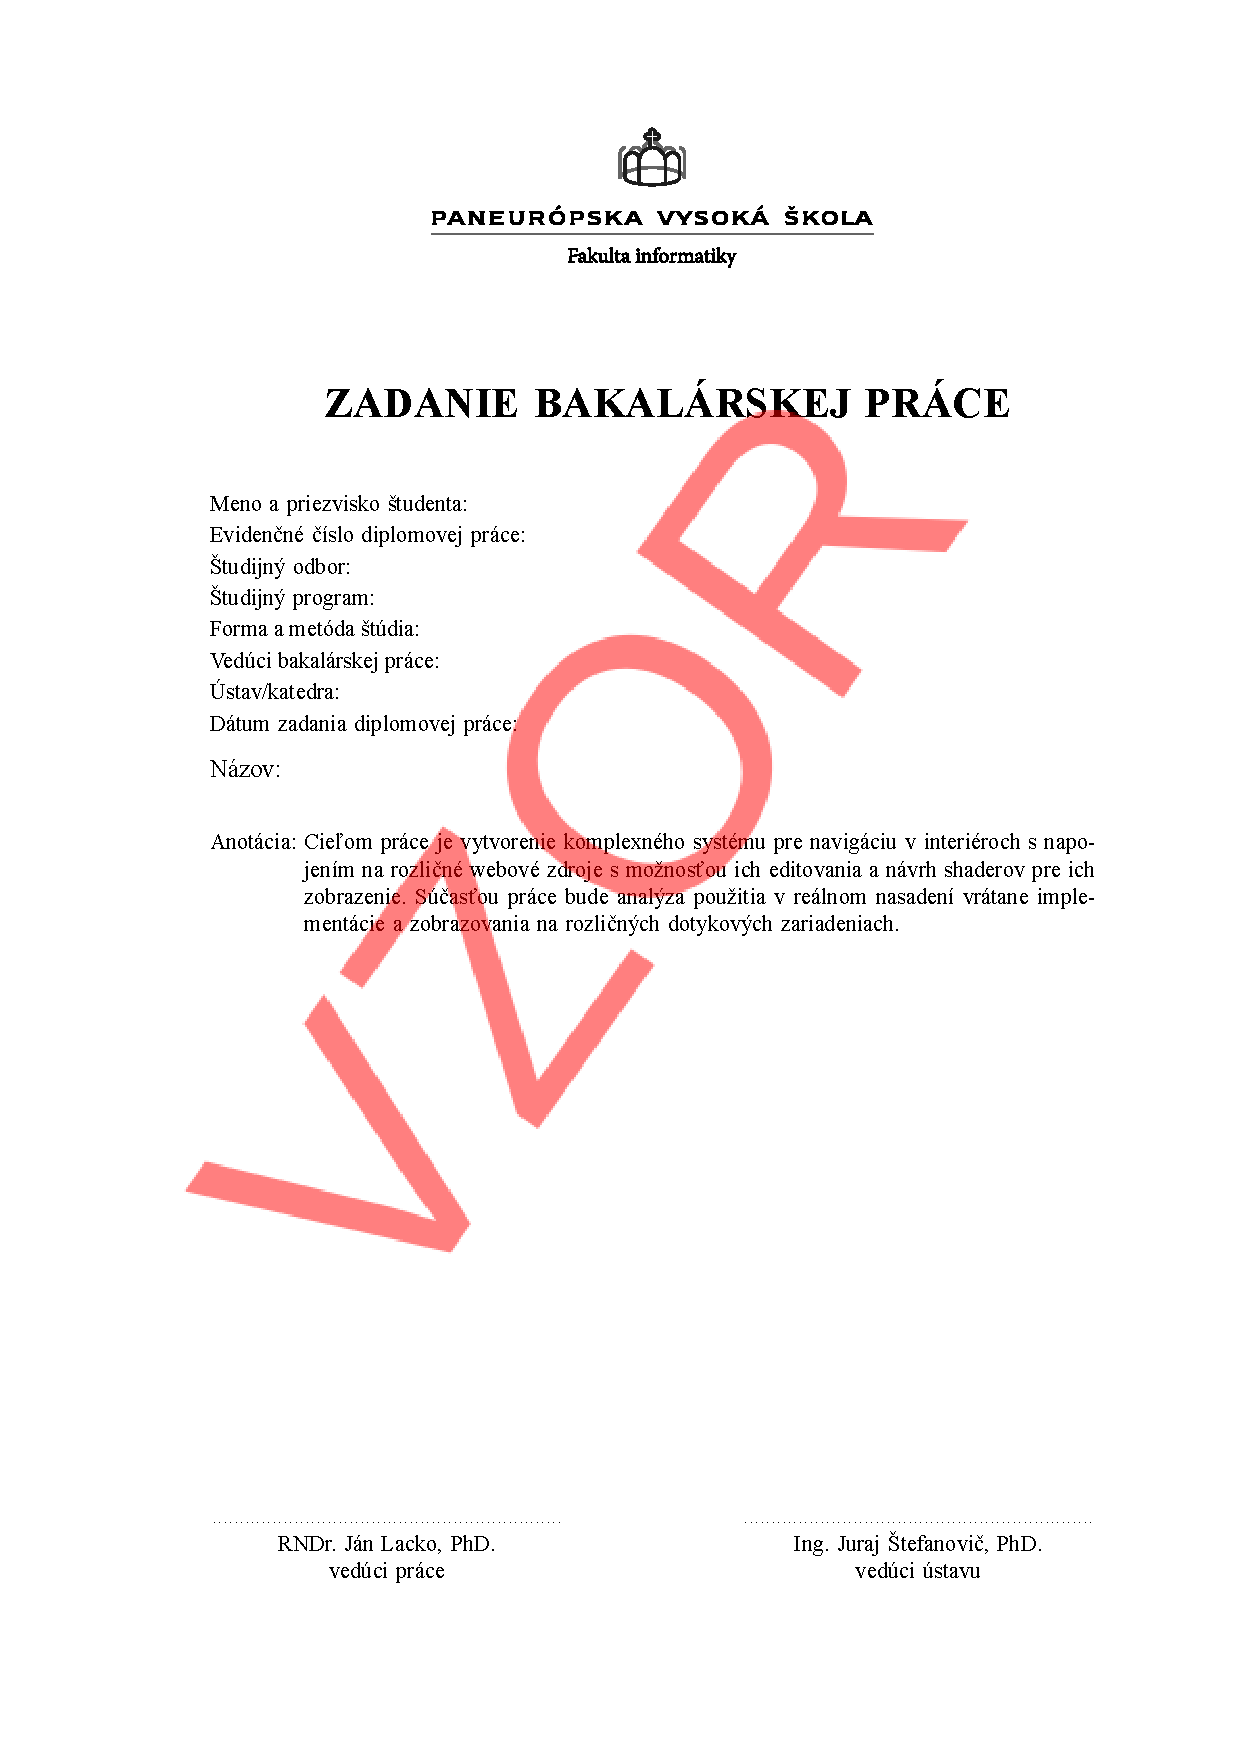
\includepdf{essentials/assignment.pdf}
%
% Customize these files:
\mbox{}
\vfill
\begin{flushleft}
    \textbf{\lnacknowledgement}\\[3.2em]
Pri vypracovaní tejto práce by som sa rád poďakoval za odbornú pomoc pánovi \supervisor, ktorý mi poskytol mnoho cenných rád a konzultácií.
\vspace{1em}\\
\small{Poďakovanie môžete napísať podľa seba.}
\end{flushleft}


\makeatletter
\vspace*{\fill}
\begin{flushleft}
    \textbf{\lndeclaration}\\[3.2em]
    \lndeclarationtext
\end{flushleft}
\vspace{1em}
\begin{flushright}
    \begin{tabular}{c}
        \makebox[50mm][c]{\dotfill} \\ % Center align the dots
        \makebox[50mm][c]{\@author} % Center align the author name
    \end{tabular}
\end{flushright}
\makeatother

\include{essentials/abstract}

% Print Table of Contents, List of Figures
\tableofcontents
\pagebreak

% set style
\pagestyle{fancy}
\fancyhead{}
\fancyfoot{}
\fancyfoot[R]{\thepage\hspace{0.4cm}} % restore numbering + ugly fix for geometry change

% Increase the right margin - as seen in the doc template
\newgeometry{left=3.5cm, top=2.5cm, right=2cm, bottom=3.85cm} 

\listoffigures
\pagebreak

% Print Glossary
\glsaddall % Optional for printing all acronyms, even if not used but (TODO:) adds a weird vertical space.
\addcontentsline{toc}{section}{\lnlistabbr}
\printglossary[type=\acronymtype,title={\lnlistabbr}]



%%%%%%% DOCUMENT BODY %%%%%%%
%%%%%%%%%%%%%%%%%%%%%%%%%%%%%
\section*{\lnintro} % Introduction is unnumbered! For numbered chapters see examples.tex
\addcontentsline{toc}{section}{\lnintro}

Lorem ipsum dolor sit amet, consectetur adipiscing elit. Integer eu lacus leo. Nulla egestas purus non dignissim tincidunt. In sit amet tellus bibendum, lobortis magna ut, sodales mi. Etiam vel eros efficitur purus ultrices vulputate et quis justo. Nunc ultrices tellus a dui mattis, eget laoreet arcu tempor. Donec vestibulum, magna ac fringilla lacinia, libero risus fringilla arcu, nec consectetur nibh justo vel sem. Quisque gravida sit amet elit ut aliquam...\par
\vspace{1em}
\noindent
V prvej kapitole je popísaný súčasný stav riešenia problematiky. Popísaná je konštrukcia takého systému, ktorý ....

\noindent
V druhej kapitole prezentujeme návrh systému ...

\noindent
V tretej kapitole sme sa zaoberali popisom implementácie systému...

% Examples:
\include{examples/examples} 

\section*{\lnconclusion} % Conclusion is unnumbered!
\addcontentsline{toc}{section}{\lnconclusion}
Nezabudnite na Záver a zhodnotenie.\\  
Cieľ bakalárskej práce bol splnený.

%%%%%%%%%%%%%%%%%%%%%%%%%%%%%
%%%%%%%%%%%%%%%%%%%%%%%%%%%%%

% Bibliography
\newpage
\printbibliography[title={\lnbibliography}]
\addcontentsline{toc}{section}{\lnbibliography}

% Appendices
\include{essentials/appendices}

\end{document}
